%\vspace{-0.5cm}
\section{Introduction}
%\vspace{-0.25cm}
 A significant progress bottleneck in the object recognition and multiview geometry applications in
the 90's was attributed to the difficulties experienced by bottom-up segmentation,
which could not produce segments sufficiently stable to be used as the
basic  matching units in these applications. A dramatic  paradigm shift,
relying not on fully segmented images but rather on a collection of features, driven by feature detectors \cite{Mikolajczyk:Tuytelaars:Schmid:Zisserman:Matas:Schaffalitzky:Kadir:VanGool:IJCV05} and descriptors, such as SIFT \cite{lowe:distinctive:IJCV04} and others \cite{Mikolajczyk:Schmid:PAMI05}, on the one hand, and significant process
in  learning methods on the other, led to a breakthrough in both of these
applications, \eg, on PASCAL for  object recognition~\cite{Felzenszwalb:etal:PAMI10}.  While modern approaches are now able to tackle a couple of hundred or so categories, experience
with  much larger datasets, \eg,  ImageNet~\cite{Deng:etal:CVPR09}
and denser datasets, \eg, the~Mammalian dataset~\cite{Fink:Ullman:IJCV08} 
casts doubt on the \textit{scalability} of these methods, as elaborated on below.

The main limiting factor concerns 
the \textit{nature of the image representation} used. Recognition  performance for methods that
rely on the appearance of local patches drops exponentially with an increase in the number of categories, with a more severe drop rate
when the database enjoys greater variation; see Figure 3 of~\cite{Griffin:Perona:CVPR08}. Similarly, image classification rates drop exponentially, \eg, from 35\% to 7\% when the number of categories goes from 200 to 10,000~\cite{Deng:etal:ECCV10}.
The same drop in recognition performance can be observed if, instead of
increasing the number of categories, the density of categories in the semantic
space is increased: Performance drops to half in going from Caltech101 to the smaller but denser 72 category mammalian dataset~\cite{Fink:Ullman:IJCV08}.
Tatu \etal\cite{Tatu:Lauze:Kimia:ICCV11} showed that  the image representation is a confounding factor
in that the equivalence class of each HOG-based representation is enormous, spanning
multiple categories (which does not show when comparing a limited number
of categories, \textit{e.g.,} an airplane against
a potted plants.) 
\begin{figure}[!t]
 \fbox{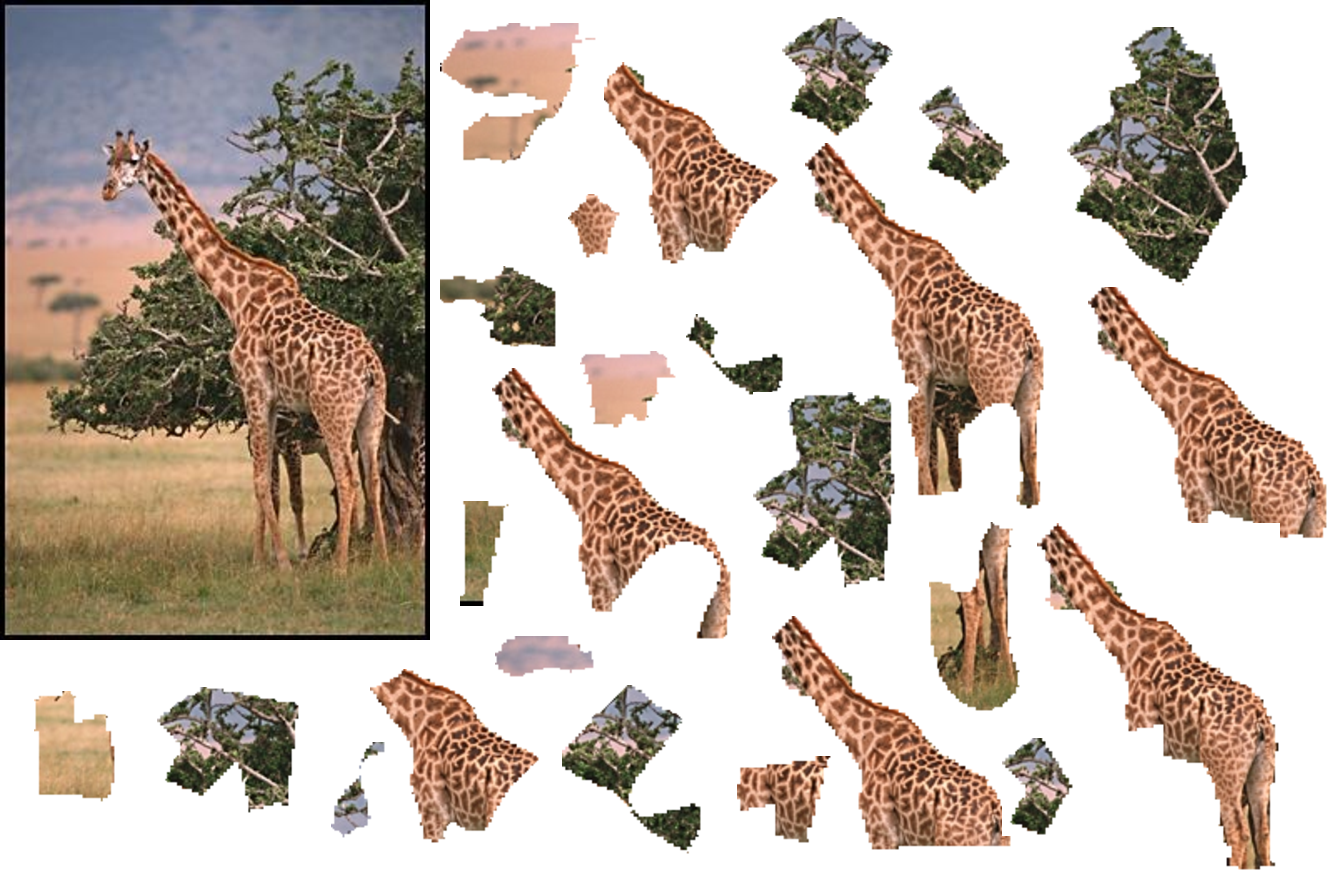
\includegraphics[height=0.148\textwidth]{figs/five_collage.pdf}}
 \fbox{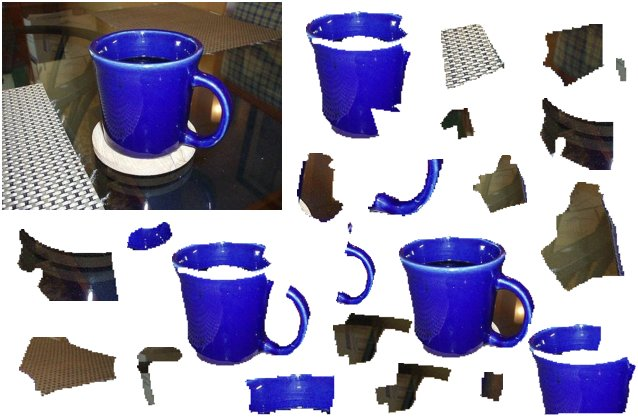
\includegraphics[height=0.148\textwidth]{figs/blue_collage.jpg}}
 \fbox{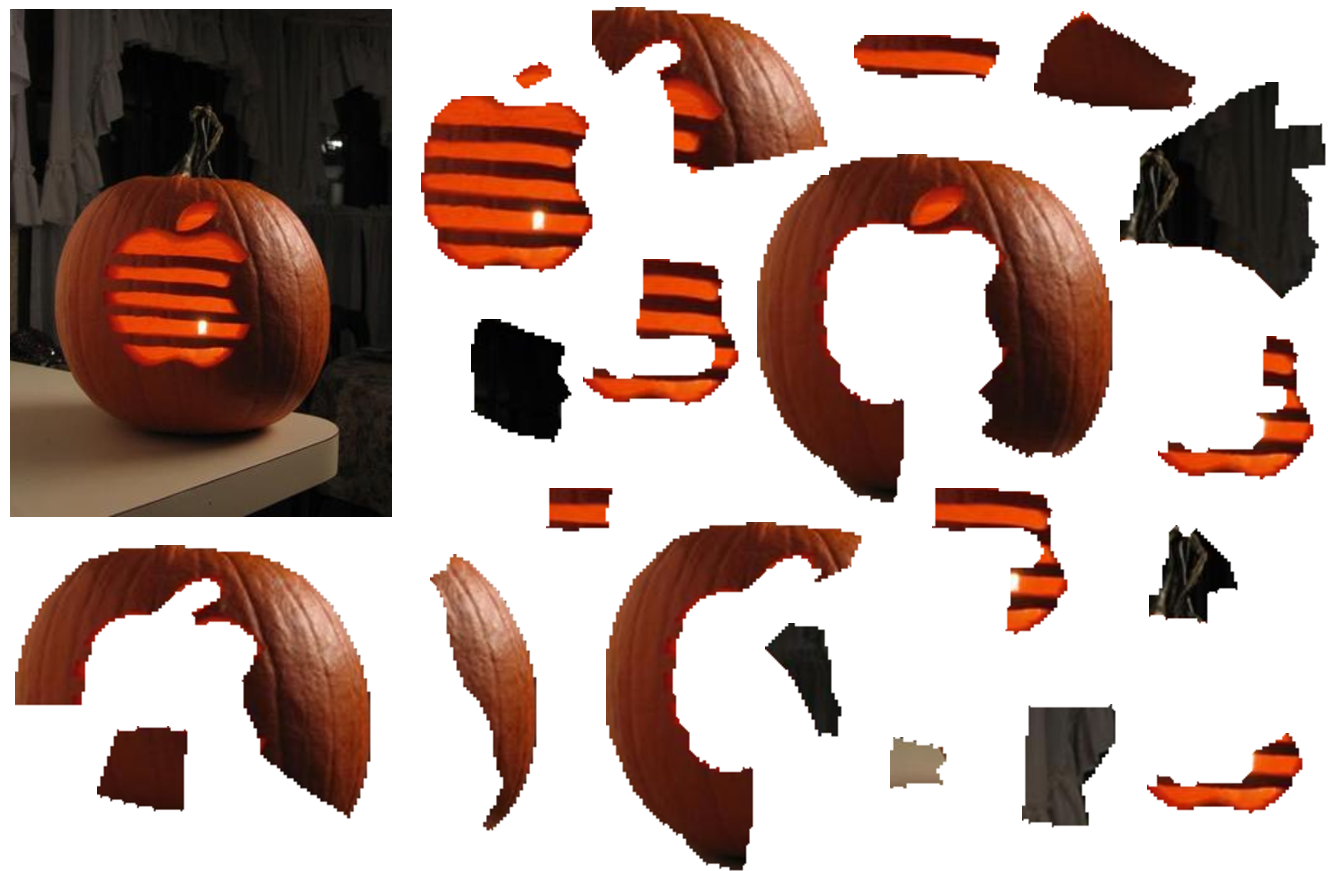
\includegraphics[height=0.148\textwidth]{figs/pumpkin_collage.pdf}}
  \fbox{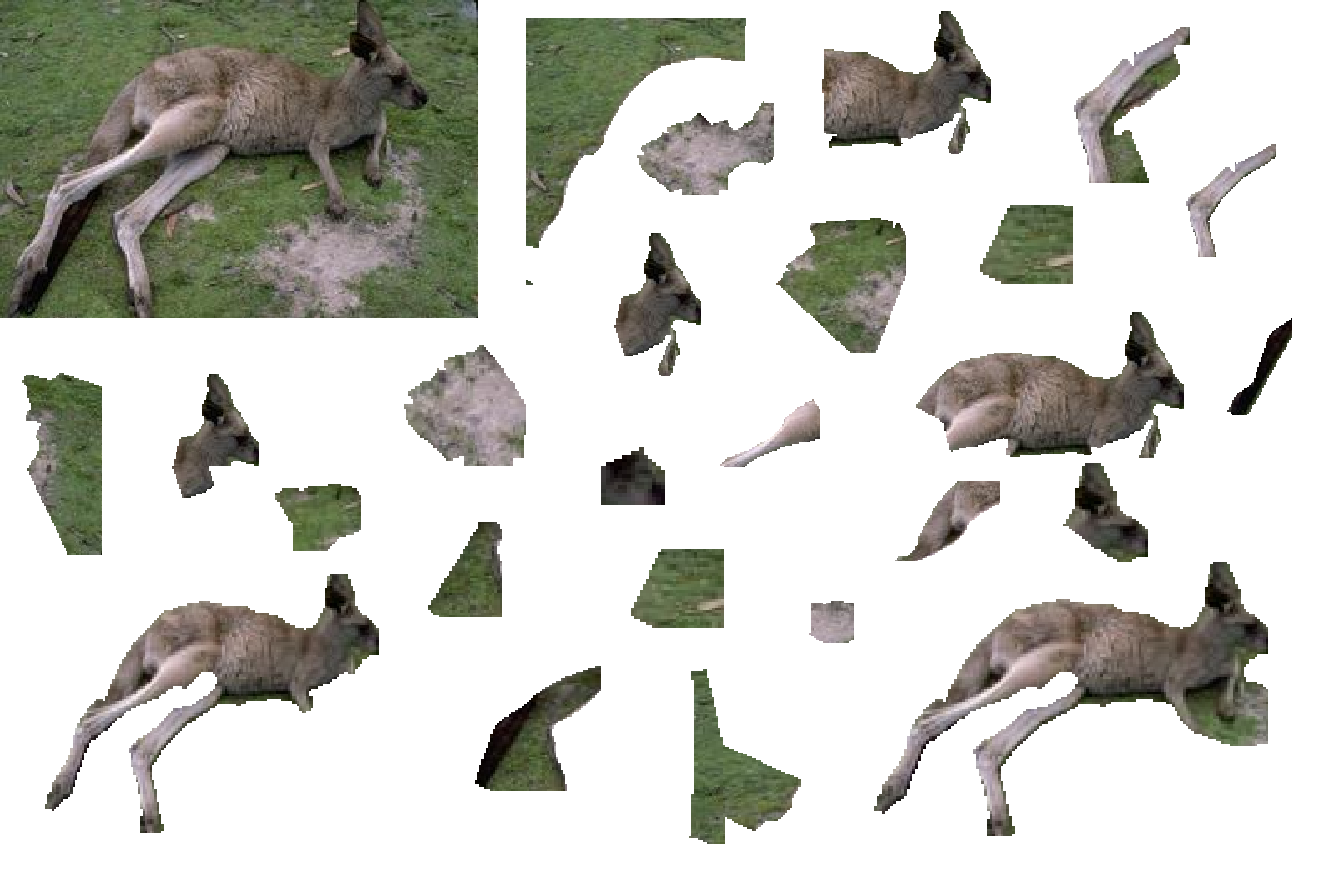
\includegraphics[height=0.148\textwidth]{figs/kangaroo_collage.pdf}} 
%\vspace{-0.25cm}
  \caption{\FigureFont A sampling of  object part hypotheses for images
from standard datasets shows recognizable fragments (in the actual fragment
set
the proportion of  
spurious fragments to recognizable ones is significantly higher, as expected).  For the rightmost figure (Berkeley dataset) we
only show the fragments that overlap with the ground truth object to show
that the parts of the object are indeed covered by our hypotheses. 
%  These preliminary results~depict a subset
% of the object part hypotheses for three  images from the ETHZ~\cite{Ferrari:etal:ECCV06} and the Brown-Extended ETHZ~\cite{Lems:Brown:ETHZ:URL}.
% Observe that in each
%  case there is at least some highly distinctive and discriminative object part hypotheses
% which are meaningful parts of the object  and  form a basis for recognition. %\vspace{-0.5cm}
 }
\label{fig:fragments:examples}
%\vspace{-0.673cm}
\end{figure}

% \begin{figure}[t]
% \label{fig:fragments:example}
% \begin{center}
%   \includegraphics[width=0.45\textwidth]{figs/giraffe_plate.pdf}
% (a)\includegraphics[width=0.45\linewidth]{figs/kangaroo.jpg}  
% \caption{This paper advocates an
% approach to forming \textit{perceptual fragments} (right), a set of conflicting and complementary
% grouping hypothesis that ensure the formation of a few meaningful object fragments in the midst of numerous background and nonsensical fragments.  It is argued that
% the distinctiveness of these fragments outweigh the expense of added clutter fragments. }
% \end{center}
% \end{figure}
% 
We posit that recognition success in these
much larger datasets critically depends on the development of \textit{more complex,  more diagnostic features} to differentiate fine-grain category differences
such as horses from
donkeys, as compared to differentiating airplanes from potted plants or
airplanes from the background in the smaller datasets. The construction of complex features when considering
a large number of categories needs to take place in a bottom-up, category independent fashion~\cite{Dickinson:CategoryBook09}. 
 Bottom-up grouping, however, requires tackling ambiguity, precisely the challenge faced by segmentation algorithms. Observe that classical
bottom-up segmentation of pixels into regions, or edges into contours,
involves
effecting a sequence of grouping actions. Even if each of these is  highly likely, a sequence of such actions is  highly likely to fail if the number of operations is large enough. Instead, it is  suggested here that \textit{all} plausible grouping operations, rather than the best local grouping, be considered and tracked to generate alternate, conflicting but complementary outcomes. This 
form of \textit{perceptual reasoning} seems intractable at first due to the apparent combinatorial explosion of possibilities. Nevertheless, it is shown here that through an effective
representation, use of multiple cues, and avoidance of duplication, the grow rate is sufficiently tamed to allow reasonable partial groupings
to form. A fraction of these groupings represent meaningful object parts and it is argued that this is all the higher level processes really
need; see Figure~\ref{fig:fragments:examples} for examples.  

The bottom-up delineation of recognizable parts of objects has distinct advantages over bounding box or rectangular fragments~\cite{Vidal-Naquet:Ullman:iccv03}: \textit{(i)} it removes the noise due to mixing foreground/background statistics, especially for complex, deformable, or articulating objects. \textit{(ii)} it reveals the natural scale of the object that is important for selecting scale of features;\textit{ (iii)} representation and recognition of object parts allows for top-down full object segmentation; \textit{(iv)} it allows for category-independent learning which is feasible over fragments
but not over pixels; \textit{(v)} allows for the discovery and learning of new objects; \textit{(vi)} improved efficiency as bottom-up fragments
are shared among multi-classes. 

The idea of organizing pixels into fragments for recognition as a precursor to this work was proposed in~\cite{Tamrakar:Kimia:POCV04}. The first practical use of multiple segmentation hypotheses was perhaps achieved in~\cite{Hoiem:etal:ICCV05}. It has also been advanced in the form of taking
advantage of segments formed from a hierarchical segmentation, \ie, from
a ``segmentation tree'' or a ``region tree'''~\cite{Todorovic:Ahuja:CVPR06,Todorovic:Ahuja:PAMI08,Arbelaez:etal:CVPR09}. The drawback of this type of an approach is that erroneously formed segments can propagate from level to level, thus preventing the formation of the veridical segments. \cite{Ozcanli:Kimia:BMVC07} used medial fragments randomly sampled in space and scale from the image shock graph to generate object part hypothesis which were then successfully used for object recognition, even without any learning. Alternatively, in the ``Soup of Segments'' approach \cite{Malisiewicz:Efros:BMVC07,Carreira:Sminchisescu:PAMI12,Endres:Hoiem:ECCV10}
a diverse set of segments is generated by inducing \textit{variations} in the segmentation procedure:
\textit{(i)} by using complementary segmentation algorithms, \textit{(ii)} by changing segmentation
parameters or seeding, and \textit{(iii)} by merging adjacent fragments.
In a more recent paper~\cite{Carreira:Sminchisescu:PAMI12}  a large number of independent binary min-cut segmentation problems are solved by starting
from  a sampling of seeds and terminals,  with different extents of foreground bias. The resulting pool of figure segments are then processed and ranked using certain regularities typical of projections of real-world objects, and a learning scheme is used to sample a diverse subset. Another recent paper
\cite{Endres:Hoiem:ECCV10} samples a set of seed regions, obtained from a hierarchical segmentation and by varying parameters in a CRF framework, 
to generate a diverse set of regions that are guided toward object segmentations by learned affinity functions; a structured learning approach is then used to rank the regions so that the top-ranked regions are likely to correspond to different objects.

Our approach is distinct in several ways:\   First,
previous work aims to generate full object hypotheses, while we aim to generate
recognizable and meaningful object part hypotheses. Second, previous work
generates multiple hypotheses by varying segmentation variables such as parameters, algorithms, seeding, {\emph{etc.,}} while we systematically and exhaustively investigate all reasonable
grouping options in a 
perceptual reasoning Gestalt framework, by asking questions like: what if these contour fragments are bridged across a gap? What if this contour fragment is spurious? These possibilities are all methodically tracked and the entire sets of options are maintained! This is an important distinction because while it is possible that viable fragments are not formed under the variations-of-variables scheme (e.g., object was too small and no seeds were initialized inside), it is much less likely that viable fragment would avoid being considered due to the structural and exhaustive nature of the proposed scheme.  

The overview of the paper is as follows. In Section~\ref{sec:atomic:fragments} we show that superpixels and contour fragments lack sufficient representation
bandwidth and instead propose   \textit{medial fragments}, which combines
aspects of both. Section~\ref{sec:transforms}
casts perceptual grouping operations,  such as gap completion, removal of spurious contours,
and others, in the form of  \textit{transforms} on the medial fragments,
with the distinct advantage of using both form and appearance in the transform.
 Section~\ref{sec:reasoning} introduces the containment graph as a mean of efficiently representing competing and alternative groupings, as a mid-level
organization and a gateway to object categorization. Section~\ref{sec:experiments} describes experiments and comparisons to related work. 



